
\documentclass[draft,linenumbers]{agujournal}\usepackage{knitr}
\usepackage[hyphens]{url}
\usepackage{amsmath}
% \draftfalse

\journalname{Earth's Future}



%












%
% set_top_vwci_count
%



\IfFileExists{upquote.sty}{\usepackage{upquote}}{}
\begin{document}
\title{Urban Water Conservation Policies in the United States}

\authors{Jonathan M. Gilligan\affil{1,2,3}, Christopher A. Wold\affil{3}, Scott C. Worland\affil{2}, John J. Nay\affil{3,4,5}, David J. Hess\affil{3,6}, George M. Hornberger\affil{1,2,3}}

\affiliation{1}{Department of Earth \& Environmental Sciences, Vanderbilt University, Nashville, Tennessee, USA}
\affiliation{2}{Department of Civil \& Environmental Engineering, Vanderbilt University, Nashville, Tennessee, USA}
\affiliation{3}{Vanderbilt Institute for Energy and Environment, Vanderbilt University, Nashville, Tennessee, USA}
\affiliation{4}{Information Law Institute, New York University, New York, New York, USA}
\affiliation{5}{Berkman Klein Center, Harvard University, Cambridge, Massachusetts, USA}
\affiliation{6}{Department of Sociology, Vanderbilt University, Nashville, Tennessee, USA}
% \affiliation{6}{U.S. Geological Survey, Nashville, Tennessee, USA}

\correspondingauthor{Jonathan M. Gilligan}{jonathan.gilligan@vanderbilt.edu}

%% Keypoints, final entry on title page.

% Example:
% \begin{keypoints}
% \item	List up to three key points (at least one is required)
% \item	Key Points summarize the main points and conclusions of the article
% \item	Each must be 100 characters or less with no special characters or punctuation
% \end{keypoints}

%  List up to three key points (at least one is required)
%  Key Points summarize the main points and conclusions of the article
%  Each must be 100 characters or less with no special characters or punctuation

\begin{keypoints}
\item Analysis of water conservation policies of 195 cities in 45 states
\item Water conservation policies correlate with both environmental and social variables
\item \replaced{Partisan voting patterns at both state and metropolitan levels account for}{Correlations with partisan voting patterns explain}
much of the variation
\added{ in policy adoption}.
\explain{Make it clear that we are talking about explaining variance (i.e., correlations), not making causal assertions.}
\end{keypoints}

%% ------------------------------------------------------------------------ %%
%
%  ABSTRACT
%
% A good abstract will begin with a short description of the problem
% being addressed, briefly describe the new data or analyses, then
% briefly states the main conclusion(s) and how they are supported and
% uncertainties.
%% ------------------------------------------------------------------------ %%

%% \begin{abstract} starts the second page

\begin{abstract}
Urban water supply systems in the United States are increasingly stressed as
economic and population growth confront limited water resources.
Demand management, through conservation and improved efficiency, has long been
promoted as a practical alternative to building Promethean energy-intensive
water-supply infrastructure. Some cities are making great progress at managing
their demand, but study of conservation policies has been limited and often
regionally focused. We present a hierarchical Bayesian analysis of a new measure
of urban water conservation policy, the Vanderbilt Water Conservation Index (VWCI),
for 195~cities in 45~states in the contiguous United
States.
This study does not attempt to establish causal relationships, but does
observe that cities in states with arid climates
tend to adopt more conservation measures.
Within a state, cities with
more Democratic-leaning voting preferences and
large and rapidly growing populations
tend to adopt more conservation measures.
Economic factors and climatic differences between cities do not correlate with
the number of measures adopted, but they do correlate with
the character of the measures, with arid cities favoring mandatory conservation
actions and cities in states with lower real personal income favoring rebates
for voluntary actions.
Understanding relationships between environmental and
societal factors and cities' support for water conservation measures can help
planners and policy-makers identify obstacles and opportunities to increase the
role of conservation and efficiency in making urban water supply systems
sustainable.
\end{abstract}


%% ------------------------------------------------------------------------ %%
%
%  TEXT
%
%% ------------------------------------------------------------------------ %%
\section{Introduction}
Cities face increasing challenges to their water supply because of complex
interactions among drought, infrastructure, population growth, land-use changes,
and other natural and human factors.
The prospect of climatic change adds to the difficulty of planning robust and
sustainable water supply systems, on account both of  increasing uncertainty
about future supply and demand for water, and also of predicted reductions in
water availability in some regions, such as the Southwestern United States
\citep{gcrp:natl.assessment.3:2014}.
For many years, advocates of soft approaches to managing water resources have
stressed the importance of improving  the efficiency with which society obtains
and consumes
the water services it requires  \citep{gleick:soft.water.paths:2002}.
Some cities and their associated water-supply systems respond to these
challenges by pursuing grand energy-intensive infrastructure projects to draw
water from distant or difficult sources. However,
many have also shown increasing
interest in the soft path, which involves
managing demand through efficiency and conservation
measures, and a number of cities have made impressive progress
\citep{fleck:fighting:2016}.

A pressing challenge is to identify the characteristics of successful
transitions toward sustainable water use and the necessary conditions for those
transitions to spread more widely.
Studies have investigated urban water conservation policies and several water
conservation indices are available, but these studies either lack comprehensive coverage
of water conservation policies or are geographically limited
\citep{hess:vwci:2017,sauri:conservation:2013,maggioni:conservation:2014}.
Recent research finds that individual perception of water scarcity and
preference for policy action to address scarcity depend not only on the actual
degree of water scarcity, but also on the person's ideological worldview
\citep{switzer:green.lenses:2016}, but it is not clear how these individual
preferences translate into policy action.

The Vanderbilt Water Conservation Index (VWCI) is an integer score representing
the number of measures that a city has taken to reduce its water demand, out of
a list of 79 possible policy actions
\citep{hornberger:hydrological.transitions:2015,hess:drought:2016,hess:vwci:2017}.
This list includes 31 requirements, such as restrictions on
lawn-watering or mandatory use of water-efficient plumbing in new construction
and renovations; and 21 rebates offered for voluntary actions, such
as purchasing water-efficient appliances.
Previously, we assessed this index and performed preliminary quantitative and
qualitative analyses on a subset of the central cities of the 22 largest
metropolitan statistical areas (MSAs) in the extended Southwestern United States
\citep{hess:drought:2016}.
That preliminary analysis found that propensity to
adopt water conservation measures depended both on characteristics
of the physical environment (precipitation) and on socio-economic and political
characteristics of the MSA (partisan voting and cost of living).

We represented the partisan political leanings of states and MSAs by the
Cook Partisan Voting Index (PVI) \citep{cook:pvi:2013}. The index measures
the difference between the percentage of the two-party vote received by
Democratic presidential candidates in a city or MSA and the percentage received
in the national election. Positive or negative values measure the
city's or state's preference for the Democratic (more progressive)
or Republican (more conservative) candidates,
respectively, relative to the national average.
Previous studies have indicated that a more Democratic-leaning PVI score is associated with higher environmental
policy adoption, including for renewable energy \citep{chupp:environ.voting:2011}
and water-conservation policies \citep{hess:drought:2016}, and conversely that a lower score is associated with
higher greenhouse gas emissions from power plants \citep{grant:environ.accountability:2017}.

Municipal water conservation policies are chosen by city officials, so it
may seem curious to measure partisan leanings with respect to presidential
elections. However, presidential votes have the advantage of providing a uniform
scale because voters across the country choose between the same candidates,
whereas the differences between Democratic and Republican candidates for
city and state positions vary considerably from one city or state to another,
with narrow ideological differences in some elections and wide differences in
others. Assessing partisan leanings in state and local
elections becomes more complicated and difficult when we consider that
the vast majority of American cities hold non-partisan city-council elections
\citep{svara:city.councils:2003} and that more than one third of state-legislature
races are uncontested by one of the major parties
\citep{klarner:state.elections:2015,ap:uncontested:2006}.
Moreover, detailed vote
counts are not readily available for municipal- and state-level elections as
they are for presidential elections. For all these reasons, presidential
voting patterns are a useful measure for gauging regional variations in partisan
leanings.
Finally, we note that the rate of split-ticket voting has declined rapidly
and consistently since the late 1980s \citep{fiorina:renationalization:2016}
and that even voters who self-identify as independent are found to align
consistently with one party or the other \citep{hawkins:motivated:2012},
so we believe that
presidential votes are good indicators for comparing the partisan leanings
that voters bring to state and local elections across the United States.

% Two important economic indicators are
% Regional Price Parity (RPP) and Real Personal Income (RPI),
% which represent, respectively,
% the cost of living of a city or state, relative to the national average
% and the average personal income in the city or state, adjusted for cost of
% living and inflation \citep{bea:rpp.methodology:2016}.
% Our previous analysis examined RPP, but here we chose to examine RPI because
% we expected that the ratio of income to cost of living would be more relevant
% than cost of living alone.
%
Our previous analysis found that the measure of Democratic-leaning voting preference (PVI)
for an MSA had, by a large margin,
the greatest predictive power for adopting water conservation measures
\citep{hess:drought:2016}.
% , with RPP having the second-greatest predictive power.
The importance of this measure
was supported by qualitative analysis, which suggested that the political
association of water conservation with general ``environmentalist'' politics
created political differences in the ways that cities respond to the physical
fact of water scarcity.

We subsequently expanded our database to the central cities in the
197~most populous MSAs in
the United States \citep{hess:vwci:2017},
which span 47 \added{states} and comprise more than half of the 382~MSAs
in the U.S.
\citep{census:population:2015}. Here, we present the first quantitative
analysis of the larger database, analyzing relationships between environmental
and societal characteristics of 195~cities across the contiguous
United States and those cities' propensity to adopt water conservation policies.
Our goal is to assess differences across MSAs that are correlated with higher or
lower levels of water-conservation policy adoption. Our analysis also
considers state-level
variables because MSA policy adoption can be strongly influenced by state-government actions,
such as the California state government's strong policy support for water conservation).
We identify which variables correlate most strongly with variations in water conservation policy
regimes and whether these
effects manifest differently when we consider specific aspects of
water-conservation policy, such as requirements and rebates.
%We find that differences in climate, political leanings of voters, and
%demographics are reflected in the number and kind of water conservation
%measures adopted by U.S. cities. Such insights
This may help water managers and policy makers to anticipate how
receptive a given city might be to adopting different conservation measures.

\section{Data and Methods}
\label{sec:data.methods}
\subsection{Vanderbilt Water Conservation Index}
%
%
%
\begin{figure}[htp]
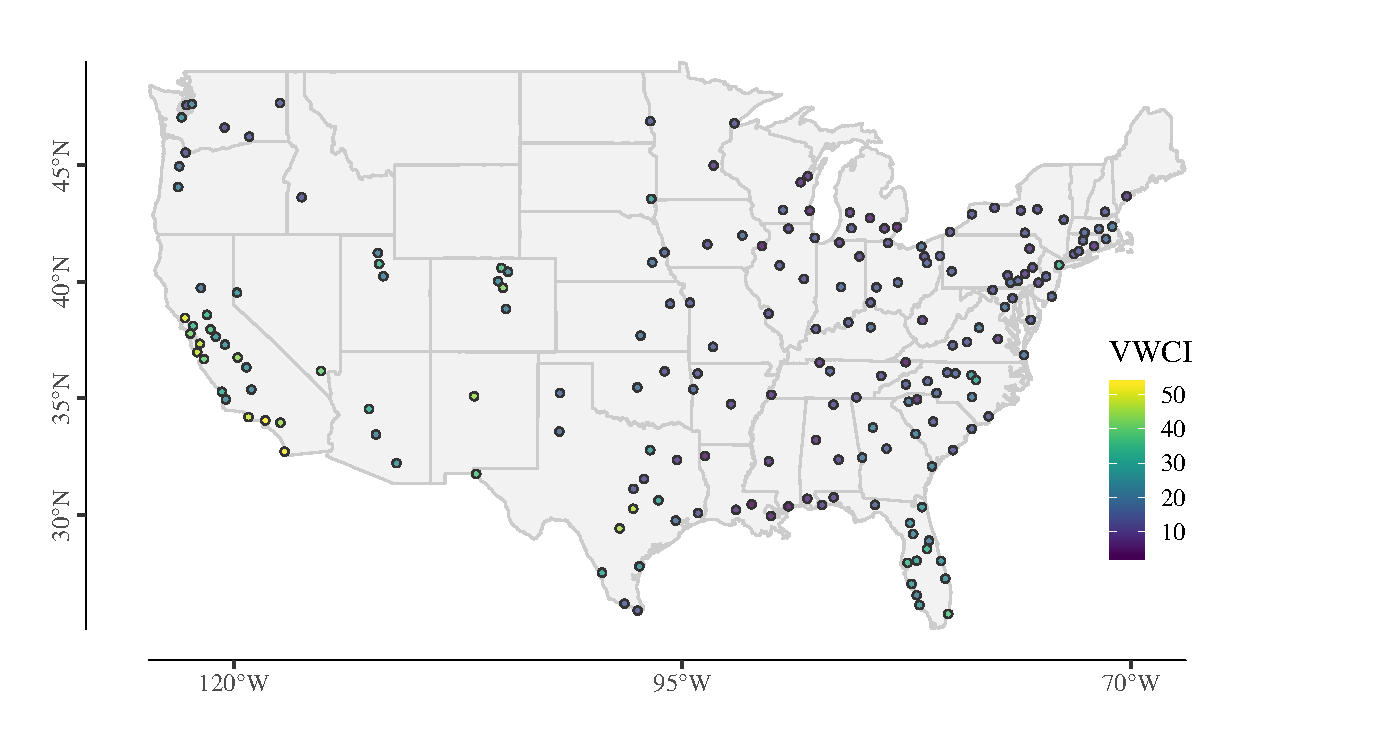
\includegraphics[width=6.5in,angle=0]{figures_clean/vwci_map-1} \caption[Map of cities with VWCI scores]{Map of cities with VWCI scores.}\label{fig:vwci_map}
\end{figure}

%
% vwci_histogram figure
%
\begin{figure}[tb]

{\centering 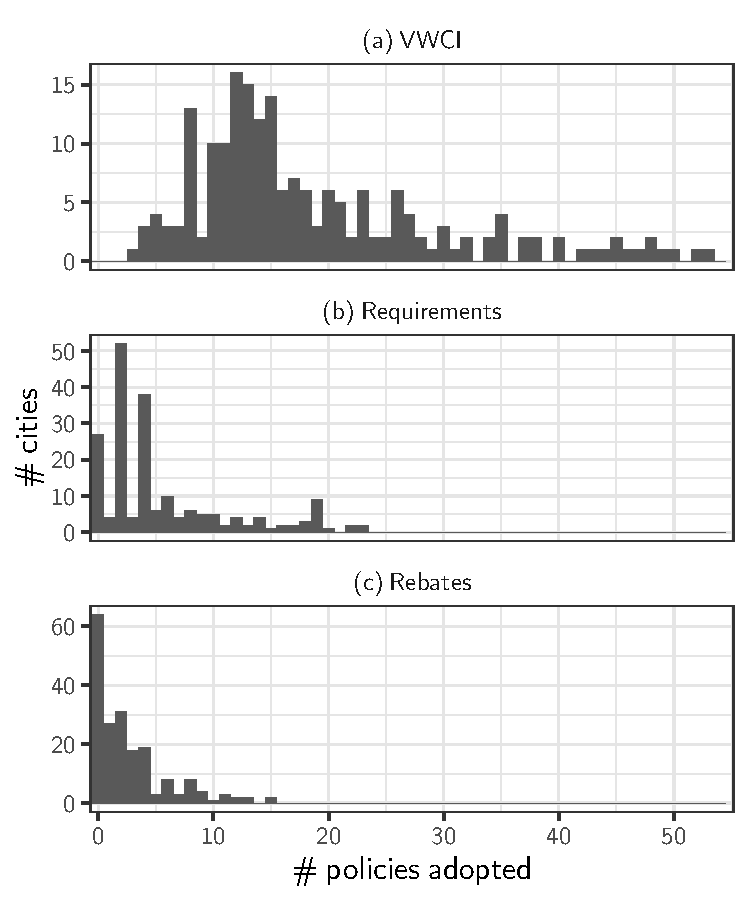
\includegraphics[width=0.8\linewidth]{figures_clean/vwci_histogram-1} 

}

\caption[Distribution of VWCI, requirements, and rebates]{Distribution of VWCI, requirements, and rebates.}\label{fig:vwci_histogram}
\end{figure}



%The VWCI data set provides detailed information about both the number and
%nature of water conservation policies in n_all_cities ~cities in
%n_all_states~states  \citep{hess:drought:2016,hess.vwci:2017}.
The VWCI data set reports both the number and
nature of urban water conservation policies, which  allows hierarchical analysis
to examine the relationships between water conservation scores and
hydroclimatological and societal characteristics at both state and MSA levels.
Our complete database includes Anchorage, AK, and Honolulu, HI, but for this
analysis we chose to include only cities within the contiguous United States
(195~cities in 45~states,
Figure~\ref{fig:vwci_map})
because both
climatic and socio-political characteristics of Alaska and Hawaii may be very
different from those of the contiguous states, and also because state-level
variables that average over the enormous area of Alaska and across the multiple
Hawaiian islands may render them less suitable for our hierarchical treatment.

VWCI scores range from~3
to~53
with a mean of  18.7
and a median of 15
(Figure~\ref{fig:vwci_histogram}a; Table~S1).
The set of 79 measures for each city makes it possible to construct different variables.
In this study, we focus on three variables: the composite VWCI of all 79 policies,
the subset of 31 requirements, and the subset of 21 rebates.
The requirement scores range
from~0
to~23
with a mean of 5.6
and a median of 4
(Figure~\ref{fig:vwci_histogram}b)
and the rebate scores range
from~0
to~15
with a mean of 2.7
and a median of 2
(Figure~\ref{fig:vwci_histogram}c).
%
% top_vwci table
%
% latex table generated in R 3.5.0 by xtable 1.8-2 package
% Wed May 16 00:29:58 2018
\begin{table}[tbp]
\centering
\caption{Cities with the twenty highest VWCI scores. Req. = requirements, Reb. = rebates. A complete list of all 195 cities appears in Table~S1.} 
\label{tab:top_vwci}
\begin{tabular}{rlrrrr}
  \hline
\multicolumn{1}{c}{ Rank } & \multicolumn{1}{c}{ City } & \multicolumn{1}{c}{ VWCI } & \multicolumn{1}{c}{ Req. } & \multicolumn{1}{c}{ Reb. } & \multicolumn{1}{c}{ $\text{Req.}/\text{Reb.}$ } \\ 
  \hline
  1 & Los Angeles, CA &  53 &  23 &  13 & 1.77 \\ 
    2 & San Diego, CA &  52 &  19 &  15 & 1.27 \\ 
    3 & Santa Rosa, CA &  50 &  19 &  15 & 1.27 \\ 
    4 & Oxnard, CA &  49 &  23 &  11 & 2.09 \\ 
    5 & San Jose, CA &  48 &  22 &  12 & 1.83 \\ 
    5 & Santa Cruz, CA &  48 &  20 &  11 & 1.82 \\ 
    7 & Austin, TX &  47 &  19 &  11 & 1.73 \\ 
    8 & San Antonio, TX &  46 &  19 &   8 & 2.38 \\ 
    9 & Albuquerque, NM &  45 &  19 &  12 & 1.58 \\ 
    9 & Riverside, CA &  45 &  15 &  13 & 1.15 \\ 
   11 & Fresno, CA &  44 &  22 &   8 & 2.75 \\ 
   12 & Denver, CO &  43 &  19 &   8 & 2.38 \\ 
   13 & San Francisco, CA &  42 &  18 &   9 & 2.00 \\ 
   14 & Las Vegas, NV &  40 &  18 &   7 & 2.57 \\ 
   14 & Salinas, CA &  40 &  19 &   6 & 3.17 \\ 
   16 & El Paso, TX &  38 &  19 &   3 & 6.33 \\ 
   16 & Miami, FL &  38 &  14 &   8 & 1.75 \\ 
   18 & Fort Collins, CO &  37 &   9 &   8 & 1.12 \\ 
   18 & Stockton, CA &  37 &  14 &   8 & 1.75 \\ 
   20 & New York, NY &  35 &  19 &   2 & 9.50 \\ 
   20 & Salt Lake City, UT &  35 &  18 &   2 & 9.00 \\ 
   20 & Tampa, FL &  35 &  14 &   5 & 2.80 \\ 
   20 & Vallejo, CA &  35 &  14 &   6 & 2.33 \\ 
   \hline
\end{tabular}
\end{table}

The 20~cities with the greatest VWCI scores are in states in the
Western U.S., with the exception of two cities in Florida and one in New York
(Tables~\ref{tab:top_vwci}, S1). Cities with similar total VWCI scores, such as
New York and Salt Lake City vs.\ Tampa and Vallejo, El Paso vs.\ Miami, and
Riverside vs.\ Fresno, may have very different relative contributions from
requirements and rebates.
Our previous qualitative research
indicated that there might be a preference for rebates over requirements in more
politically conservative cities \citep{hess:drought:2016,brown:politics:2016}.
Consequently, in addition to the VWCI score we also analyzed the number of
rebates and the number of requirements in a city's portfolio of conservation
policies.

The relative contributions of rebates and requirements to VWCI varied
considerably (Tables~\ref{tab:top_vwci}, S1)

\subsection{Explanatory Variables}
We selected explanatory variables with the goal of understanding the
relative contribution of political-economic and hydroclimatological factors
to policy adoption.
We selected one political variable (the Cook Partisan Voting Index, PVI) for reasons
described above and one economic variable (\replaced{relative}{real} personal income, RPI).
We calculated PVI using state- and county-level presidential votes averaged over the
2008 and 2012 elections \citep{cook:pvi:2013,cq:elections:2016}
(Tables~S1--S2 and Datasets~S1--S4).
Positive PVI indicates that the Democratic share of the two-party vote was greater
than the national average, and negative PVI indicates a greater Republican vote share.
Income is generally correlated with education and with a range of other variables that
are associated with differences in policy adoption, and we reasoned that in poorer
regions there may be a preference for rebates and other optional policies.
We chose real personal income (RPI), which represents the average personal income in the city
or state, adjusted for inflation and the regional cost of living
\citep{bea:rpp.methodology:2016}.
We obtained RPI for MSAs and states in 2014 from the
\citet{bea:rpi:2016}.

For the \replaced{hydrological}{hydroclimatological} variables, we
obtained values for the MSA-level monthly average temperature ($T$) and monthly
total precipitation ($P$) for the period 1900--2014 from the University of Delaware's
gridded climate reanalysis
\citep{matsuura:gridded.temp:2015,matsuura:gridded.precip:2015}
and for state-level from the National Climatic Data Center's divisional temperature
and precipitation records for the Continental U.S.
\citep{vose:nclimdiv:2014}.
We calculated the mean annual temperature and precipitation over a
30-year interval from 1985--2014.
We obtained the fraction of the public water supply taken from surface water sources
(henceforth, surface-water fraction) from the U.S. Geological
Survey's water use report for 2010 \citep{maupin:water.use:2014}.

In addition to the two political-economic variables and the two hydroclimatological variables,
we included measures for total population and population growth of the MSA. Our previous research had
indicated that larger cities have more capacity to adopt water-conservation policies and that more
rapidly growing cities are more concerned with water supply. We obtained populations for MSAs and states
in 2010 and 2014 from the \citet{census:population:2015} and used them to calculate average annual rates
of population growth.

We began with the covariates listed above, but adopted a modified set based on
preliminary results: The regression coefficients for $T$ and $P$ showed
collinearity.
This, together with a desire for parsimony, led us to replace them with the
K\"oppen aridity index: $P / (T + 33)$, with $P$ in millimeters and $T$ in
Celsius.
The K\"oppen index is
derived from mean annual temperature and precipitation
and correlates reasonably well with other aridity indices
that incorporate evapotranspiration
\citep{quan:aridity:2013}.
Larger values of this index correspond to wetter conditions
and smaller values to drier conditions.

The distribution of MSA population in~2014 was skewed, with
a few large cities producing an asymmetric fat tail (Figure~S1),
so we deemed the natural logarithm of population
a more suitable predictor
for a regression analysis \citep[pp.~59--61]{gelman:arm:2007}.

\subsection{Regression Analysis}
We applied Bayesian hierarchical varying-intercept
logistic regression to each of the
three conservation scores (VWCI, number of requirements, and number of rebates)
with the following explanatory variables:
PVI (Democratic Party preference), RPI (real per-capita income),
the K\"oppen aridity index, surface water fraction,
metropolitan population, and population growth rate.
The hierarchical structure of our regression model, which nests cities and MSAs
within states, reflects the fact that water resources extend beyond MSA
boundaries and that state-level policies affect local actions, both by
constraining local ordinances and regulations, and by encouraging or requiring
counties and cities to adopt various types of conservation measures.
We also considered a hierarchical varying-slope model, but with an average
of only 4.3 MSAs per state there were too few degrees of freedom to adequately
constrain 6 additional regression coefficients for each state.

The regression analysis follows standard textbook treatments
\citep{gelman:arm:2007,gelman:bda:2014}.
Each city's water-conservation score (VWCI, requirements, or rebates) is
an integer count out of a maximum number of possible actions.
We model this as a quasi-binomial process, in which each policy action
for city $i$ is adopted independently, with
the $m$\textsuperscript{th} action, $a_m$, having probability
$p_{im}$.
In a pure binomial process, each policy in city $i$ would have the same
probability $p_i$ of being adopted.
The variance of a pure binomial distribution is uniquely determined
by its mean and the variance of the VWCI data was
greater than a pure binomial
distribution could account for,
so our model uses a beta-binomial process, which allows for greater dispersion
of scores by drawing the probabilities $p_{im}$
for the different actions in city $i$ from a beta distribution with mean $p_i$
\citep[pp.~437--38]{gelman:bda:2014}.

We model the cities' mean probabilities $p_i$
with a hierarchical varying-intercept logistic
regression in which MSAs are nested within states and
water-conservation policy measures
are associated with both
state-level and MSA-level covariates.
For city $i$, located in state $j$,
\begin{linenomath*}
\begin{align}
\text{Score}_i \sim{}& \text{beta-binomial}(N_{\text{action}}, \phi p_i, \phi (1 - p_i)), \\
\intertext{where}
p_i ={}& \text{logit}^{-1}(y_i),\\
y_i ={}& \alpha_{j} + \sum_{k \in \text{MSA variables}} \beta_k x_{ik}, \label{eq:y}\\
\alpha_{j} ={}&
\alpha_0  + \sum_{k \in \text{state variables}} \gamma_k w_{jk} + \delta_{j},
\end{align}
\end{linenomath*}
$N_{\text{action}}$ is the number of possible conservation actions
(79 for VWCI, 31 for requirements, and
21 for rebates),
$\beta$ is a vector of MSA-level regression coefficients,
$x$ is a matrix of MSA-level covariates,
% ($x_{i,j}$ is the $j$th covariate for city $i$),
% $\text{state}_i$ represents the state of city $i$,
and $\alpha_j$ is the intercept of the MSA-level regression
for all cities in state $j$.
%and $\epsilon_i$ represents random noise at the MSA-level, which we do not explicitly model.
We do not include a noise term in Equation~\ref{eq:y} because random variations
related to the probabilities $p_i$ are incorporated in the beta-binomial
process \citep[p.~321]{gelman:arm:2007}.
The inverse logit function maps the real numbers onto the interval $(0,1)$,
thus transforming $y_i$ to a probability.
The overdispersion of conservation scores is parameterized by $\phi$:
as $\phi \rightarrow \infty$, the distribution of conservation scores approaches
a binomial distribution, and the smaller $\phi$ is, the greater the
overdispersion.

In modeling $\alpha_j$,
$\alpha_0$ is the mean intercept across all states,
$\gamma$ is a vector of state-level regression coefficients,
$w$ is a matrix of state-level covariates,
% ($w_{\text{state}_i,k}$ is the $k$th covariate for the state of the $i$th MSA),
and
$\delta$ is a random noise term that represents state-level variations not
accounted for by the regression model.
%$\sigma$ is a scale parameter for $\delta$.
We constrain $\delta$ to sum to zero in order to keep the model identifiable
\citep[Ch.~23]{stan:manual:2015}.

\replaced{Standardizing}{We standardized the} independent variables \added{$x$ and $w$} to put them on a common
scale\added{. This}\explain{Break up long sentence for clarity, and replace passive voice with active.} serves both
to facilitate comparing the relative importance of variables whose natural scales are
vastly different
\citep[pp.~55--57]{gelman:prior:2008,gelman:arm:2007},
and also to improve computational performance \citep{stan:manual:2015}.
\replaced{State-level covariates were rescaled}{We rescaled the state-level covariates} to have means of zero and
standard deviations of 0.5, as recommended by \citet{gelman:prior:2008}
and \citet[pp.~55--57]{gelman:arm:2007}:
$w_{\text{scaled}} = (w - \mu_w) / (2 \sigma_w)$,
where $w$ is a state-level covariate,
$\mu_w$ is the mean over all states,
and $\sigma_w$ is the standard deviation over all states.
Where the same covariate appeared at both the state and
MSA level,
we addressed multicollinearity between state-level and MSA-level
variables by rescaling the MSA-level covariate
to the same scale as its state-level counterpart and
subtracting the state-level value,
so that MSA-level covariate represented the difference between the MSA and
the state-average:
$x_{\text{scaled}} = (x - w) / (2 \sigma_w)$, where $x$ is an MSA-level
covariate, $w$ is the state-level covariate for the MSA's state, and $\sigma_w$
is the standard deviation of $w$ over all states.
Covariates that only appeared at the MSA level were rescaled so
the mean over all 195~MSAs was zero and the standard deviation~0.5:
$x_{\text{scaled}} = (x - \mu_x) / (2 \sigma_x)$, as above.

We recognize that there are various ways that the multilevel model could be
configured.
Our choice of models was based on the theoretical objective of highlighting MSA-level
difference in water-conservation policies. This choice involved three decision criteria.
First, we selected the four main variables (Democratic-leaning, income, aridity, and
surface water) on theoretical grounds described above with our goal of understanding the
relative strength of political and economic factors and hydrogeological factors. The
population variables were included as ``controls.'' This choice of variables allowed us to
have a balanced approach to sociohydrological factors and to show that policy adoption is
not a simple outcome of hydrological factors. Second, we selected the state-government
level as the higher level for the model because water conservation policy is frequently
driven by state-government organizations and policies. Third, any of the four variables
could be included only at the MSA level rather than at both the MSA and state levels, but
doing so would tend to bias the model toward an overestimation of MSA-level differences.
By using a model that includes these four variables at both the MSA and state levels, and
by normalizing the MSA-level variables to state averages, we developed a conservative
approach to showing the importance of MSA-level differences.
Thus, when we demonstrate MSA-level differences, we do so with a model that would tend
to underestimate those differences.

Because there are no previous quantitative comprehensive analyses of urban
water conservation policies, we represent our ignorance at the outset by
choosing weakly-informative priors, so the regression results are almost
entirely determined by the data, and are only weakly constrained by the priors.
We follow \citet{gelman:prior:2008}'s analysis
of weakly-informative priors for logistic regression
by choosing Cauchy priors with a scale of 2.5 for the
parameters corresponding to the standardized variables ($\alpha_0$, $\beta$,
and $\gamma$).
We represent $\delta$ as normally distributed
with a scale defined by the hyperparameter $\sigma$ with a positive half-Cauchy
hyperprior \citep{gelman:prior:2008}.
For $\phi$, we parameterized the Cauchy priors
\emph{ad-hoc}, based on the data, and setting the scales by trial and error
to make the prior distribution wide enough that it did not noticeably constrain
the posterior.
\begin{linenomath*}
\begin{align}
\alpha_0, \beta, \gamma \sim{} & \text{Cauchy}(0,2.5),\\
\delta \sim{}& \text{normal}(0,\sigma),\\
\sigma \sim{}& \text{positive half-Cauchy}(0,2.5),\\
\intertext{and}
\phi \sim{}& \begin{cases}
\text{Cauchy}(50,20) & \text{for VWCI}. \\
\text{Cauchy}(15,10) & \text{for requirements and rebates}. \\
\end{cases}
\end{align}
\end{linenomath*}

We implemented the statistical model in the Stan probabilistic programming
language \citep{carpenter:stan:2016}, which generates a Hamiltonian Monte Carlo
sampler.
We used R to prepare the data and call the sampler \citep{r.manual:2016}.
We
sampled four Markov chains for 1000 iterations each, after 1000 warm-up iterations,
which yielded a total of 4000 samples.
% where each sample is a vector containing a value for each of the model paraameters.
% These samples approximate random draws from the joint posterior probability
% distribution for the parameters, given the priors and the data,
% so the statistics of the samples approximate those of the
% posterior distribution.
The means and medians of the posterior distributions for
regression coefficients $\beta$ and $\gamma$, were equal within $\pm 0.01$
(Tables~S15--S17).
Code to reproduce the analysis is included in the supporting information.

To facilitate interpretation, we
follow the recommendations of \citet[pp.~81--82]{gelman:arm:2007} by reporting
rescaled regression coefficients:
\iffalse
$\beta' = N_{\text{action}} \beta / 4$ and $\gamma' = N_{\text{action}} \gamma / 4$,
which represent the approximate change in VWCI (or requirements or rebates)
\else
$\beta' = \beta / 4$ and $\gamma' = \gamma / 4$, which represent
the approximate change in the probability $p$
\fi
corresponding to
a two-standard-deviation change of the covariate near the
midpoint of the logistic function (where $p = 0.5$).
The corresponding change in VWCI, requirements, or rebates
of
$\beta' N_{\text{action}}$ or $\gamma' N_{\text{action}}$.
For example, $N_{\text{VWCI}} = 79$,
so if $\beta'_k = 0.1$ for some covariate $x_k$,
then for a city
with VWCI of 39 ($p \approx 0.5$),
a two-standard-deviation change in $x_k$ would correspond
to a change in VWCI of roughly 8.

We tested VWCI for overdispersion by comparing binomial and beta-binomial models
using leave-one-out cross-validation (LOO)
(Tables~S3--S5),
the Widely Applicable Information Criterion (WAIC)
(Tables~S6--S8),
and also by visual inspection of the distribution of posterior predictions of
the mean, standard deviation, maximum, and minimum of VWCI over the cities in
our data set \citep{gelman:bda:2014,gelman:predictive:2014,vehtari:loo:2016}.
All three methods favored the overdispersed beta-binomial model.
These tests also strongly favored a
hierarchical
model over a single-level regression on MSA-level covariates.

\section{Results}
With respect to the political-economic variables, regressions
for VWCI, requirements, and rebates
(Figure~\ref{fig:vwci_cat_plot}; Tables~S15--S17)
all show correlations between
adoption of water-conservation policies and Democratic-Party vote share
at both the state and MSA levels.
States with greater Democratic-leaning PVI scores have greater propensity to adopt conservation policies,
as do MSAs with greater Democratic vote-share than the rest of the state.
Personal income (RPI) does not correlate meaningfully with the conservation indices at the state level, except in the
case of rebates, and it is negligible at the MSA level.
With respect to the hydroclimatological variables, state-level
aridity also correlates with all three conservation scores
with MSAs in drier (low-aridity) states having a greater propensity for conservation.
Variations of aridity from one MSA to another within a state have a pronounced
correlation with requirements, but not with VWCI and rebates.
Surface-water dependence does not correlate meaningfully with the conservation indices
at the state or MSA levels.

At the MSA level, faster population growth and larger population correlate with higher values
for all three conservation scores.
This finding was expected for reasons given above.
%
% vwci_cat_plot
%
\begin{figure}[p]

{\centering 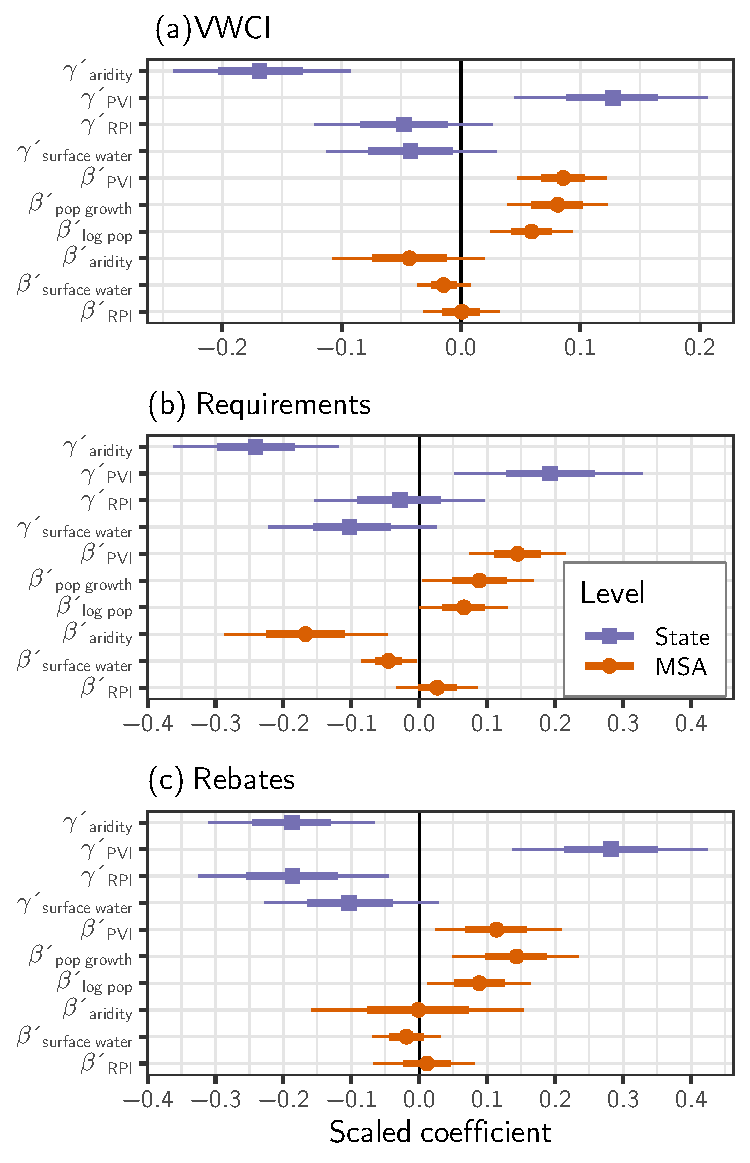
\includegraphics[width=0.8\linewidth]{figures_clean/vwci_cat_plot-1} 

}

\caption[Scaled regression coefficients for VWCI, requirements, and rebates]{Scaled regression coefficients for VWCI, requirements, and rebates: $\gamma$ refer to state-level regression coefficients and $\beta$ to MSA-level ones.
%Coefficients are scaled  so the value on the horizontal axis represents the approximate change in the probability $p_i$ of adopting an action, corresponding to a  two-standard-deviation change in the predictor when $p_i$ is around 0.5.
For a scaled coefficient of 0.1, a two-standard-deviation change in the predictor corresponds to VWCI changing by about 8 for a city with a VWCI of around 40, the number of requirements changing by about 3 for a city with around 16 requirements, and the number of rebates changing by about 2 for a city with around 10 rebates. The points represent the median of the posterior, the thick lines the 66\% highest-density interval (HDI), and the thin lines the 95\% HDI. Coefficients are grouped by state vs. city level and then ordered within each group by absolute value of the median for the VWCI analysis.}\label{fig:vwci_cat_plot}
\end{figure}


For all three conservation scores, the largest \replaced{correlations}{effects}\explain{To be precise, this paragraph discusses effect sizes, not correlation coefficients.} were for state-level,
as opposed to MSA-level, characteristics, but the posterior distributions show
considerable overlap so it is important not to over-interpret the ranking of
coefficients.

Two differences that stand out among the three measures are that state-level
variation in real personal income (RPI) and MSA-level variation in aridity
do not correlate meaningfully with
total VWCI. However, they do
correlate differently with
requirements versus rebates:
state-level real personal income
correlates more strongly with rebates
than with requirements
and MSA-level variations in aridity
correlate more strongly with requirements
than with rebates.

%
% vwci_residual_range
%

Regression residuals for VWCI range
from $-15.2$
to~$+17.1$,
with a root-mean-square value of
$5.3$
(Figure~\ref{fig:vwci_residuals} and Table~\ref{tab:vwci_top_residuals}).
There is no indication of multicollinearity creating worrisome correlations
among the coefficients (Figures.~S2--S4).
%
% vwci_residuals
%
\begin{figure}[tb]

{\centering 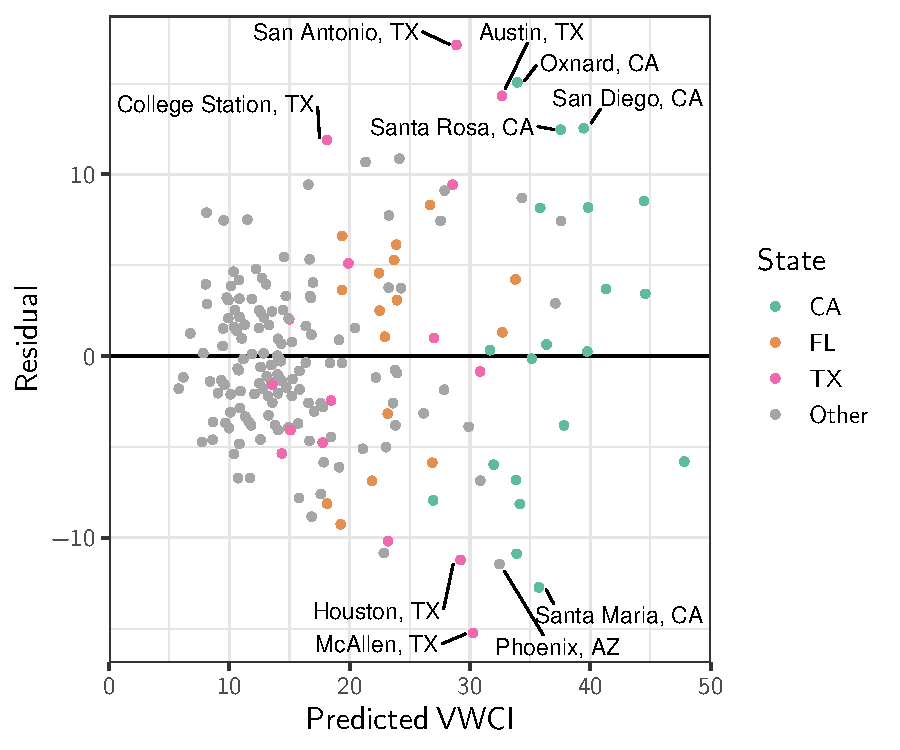
\includegraphics[width=0.8\linewidth]{figures_clean/vwci_residuals-1} 

}

\caption[Predicted versus actual VWCI]{Predicted versus actual VWCI. Cities with the ten largest residuals are labeled. Cities in California, Florida, and Texas are indicated by color (these states contain 27\% of the MSAs in our data set)}\label{fig:vwci_residuals}
\end{figure}

%
% vwci_top_residuals
%
% latex table generated in R 3.5.0 by xtable 1.8-2 package
% Wed May 16 00:30:04 2018
\begin{table}[tbp]
\centering
\caption{Cities with the ten largest residuals from VWCI regression.} 
\label{tab:vwci_top_residuals}
\begin{tabular}{rlrrr}
  \hline
\multicolumn{1}{c}{ Rank } & \multicolumn{1}{c}{ City } & \multicolumn{1}{c}{ VWCI } & \multicolumn{1}{c}{ predicted VWCI } & \multicolumn{1}{c}{ residual } \\ 
  \hline
 1 & San Antonio, TX & 46 & 28.9 & 17.1 \\ 
   2 & McAllen, TX & 15 & 30.2 & $-$15.2 \\ 
   3 & Oxnard, CA & 49 & 33.9 & 15.1 \\ 
   4 & Austin, TX & 47 & 32.7 & 14.3 \\ 
   5 & Santa Maria, CA & 23 & 35.7 & $-$12.7 \\ 
   6 & San Diego, CA & 52 & 39.5 & 12.5 \\ 
   7 & Santa Rosa, CA & 50 & 37.5 & 12.5 \\ 
   8 & College Station, TX & 30 & 18.1 & 11.9 \\ 
   9 & Phoenix, AZ & 21 & 32.4 & $-$11.4 \\ 
  10 & Houston, TX & 18 & 29.2 & $-$11.2 \\ 
   \hline
\end{tabular}
\end{table}



\subsection{Robustness checks}
As described above, we chose our explanatory variables
for theoretical reasons with the goal of understanding the relative role of political-economic
and hydroclimatological differences among MSAs as factors that explain water-conservation policy
adoption.
To test the robustness of our analysis,
we compared the results described above to three kinds of alternate regression
analyses for the VWCI
(See discussion of robustness, Figures~S5--S10, and Tables~S3--S14
in Supporting Information).
\explain{Explain how we compared different models.}%
\added{We compared the predictive accuracy of the different analyses using information-criteria scores
\citep{gelman:predictive:2014,vehtari:loo:2016}
and also considered whether the regression coefficients produced by the alternate were substantively
different from those of the original analysis.}

First, we tested whether conservation policies might be more
responsive to recent extreme events, such as drought, by varying the
period over which we averaged the aridity index.
Both the regression coefficients and the information criteria were
indistinguishable for the different averaging periods
\added{(Figure S5 and Tables S3 and S6)}.

Second, we repeated the regression analysis
with different sets of covariates:
substituting MSA population density
for the total population or
including the MSA area and Gini index of income inequality as additional
predictors (Figure~S6, Tables~S4 and~S7).
In all of these analyses, regression coefficients $\beta$ and $\gamma$
were consistent with the original model.
The information criteria were also consistent with one another.
In all of these analyses, the original set of covariates received the best
scores by a small\deleted{ and insignificant}%
\explain{Moved discussion of uncertainty to the next paragraph.}
margin.

We also repeated the regression analysis removing either PVI or aridity
(Figure~S7, Tables~S4 and~S7).
Removing either of these covariates
\replaced{did not significantly change
the regression coefficient of the remaining covariates, and the information
criteria scores were worse in both cases.}{reduced the quality of fit to the observations,
as indicated by information criteria scores.
The models with PVI removed showed the worst quality, which indicates that PVI
made the greatest contribution to the quality of the fit and had the greatest predictive power
of the covariates we considered.
It is important to note that there was considerable uncertainty in the information criteria estimates, which makes it
difficult to disentangle the specific contributions of each covariate.
Therefore, we used information criteria scores primarily to compare the overall predictive accuracy of different
model configurations \citep{gelman:predictive:2014}.}%
\explain{Be clearer about how we compared model quality and add explanatory text for non-statisticians.}

In addition to comparing different choices of covariates, we also
examined different structures for the regression models:
In addition to hierarchical regression models that nest MSAs within states,
with different intercepts for different states, we also
considered single-level models that considered only MSA-level covariates and
used the same intercept for all MSAs,
we considered interaction terms between aridity and PVI at both
the state and MSA levels (Figure~S7, Tables~S4 and~S7),
and we considered an alternative normalization
in which the MSA-level covariates were scaled separately
from the state-level covariates to have zero mean and 0.5 standard deviation
across all MSAs ($x_{\text{scaled}} = (x - \mu_x) / (2 \sigma_x)$),
rather than representing
the scaled difference between the MSA value and the state-level value
(Figures~S8--S10, Tables~S9--S14).

The information-criteria scores for the single-level models were much
worse than for the hierarchical ones.
The interaction terms did not produce any
important changes in the other regression coefficients, and yielded
slightly (but insigificantly) worse information-criteria scores.

The alternate normalization scheme produced posterior estimate for the
coefficient of state-level PVI whose median was one third as great as for the original
normalization and consistent with zero (Figures~S8--S10).
We found an 85\% posterior probability that the coefficient of the state-level PVI
is positive in the alternative normalization, which is suggestive but inconclusive.
None of the other coefficients changed much.
The information criteria for the alternate normalization were
\replaced{slightly, but not significantly, smaller than for}{slightly inferior to}%
\explain{Clarify.}
the original normalization (Tables~S9--S14),
\replaced{so the}%
{but the difference was negligible. The}
MSA-level PVI remains important in both schemes,
but it is ambiguous whether it is
better to interpret the data as indicating that both the state-level PVI
and the difference between the state-level and MSA-level PVI are independently
correlated with water conservation policies, or whether the state-level PVI
is not correlated with conservation policies, but the MSA-level PVI is.
However, we do not think this ambiguity has much practical significance
because both models yield similar predictions for propensity to adopt
water conservation policies in a given MSA and both find an important
correlation with political preferences, although they differ on the importance
of state-level preferences.

Finally, we tested for sensitivity to the functional form of the prior
distributions and found only small and insignificant changes when we
changed scales or replaced Cauchy priors for $\alpha$, $\beta$, and
$\gamma$ with normal priors.

We conclude from these robustness checks that
except for the regression coefficient for state-level PVI
the results
of our analysis are robust against many changes of time-spans,
explanatory variables, model-structures, and assumptions about priors
and model specifications.
Across all of these variations, the political variable measuring
vote-shares for Democratic versus Republican presidential candidates,
the hydroclimatological variable measuring aridity, and the
MSA-level population and population growth rates were
consistently and strongly correlated with conservation.

There are myriad other potential explanatory variables,
but we worried that exploring a large set of alternative models
and choosing the one that performs best might
unintentionally become an exercise in ``$p$-hacking'' due to
``garden of forking paths'' effects \citep{gelman:forking.paths:2014}.
Because of these concerns, we chose to confine our analysis to the original set
of variables, which we chose for theoretical reasons
\citep{hess:drought:2016}.

\section{Discussion}

This analysis identifies distinguishing characteristics of cities across the
contiguous United States that embrace water conservation policies, and allows us
to differentiate state-level from MSA-level effects. We find that water
conservation is associated both with characteristics of the physical environment
and with political and demographic
%, and economic
characteristics of cities and states.
This finding suggests the importance of interdisciplinary thinking and
analysis in the study of water-conservation policy. The assumption that
water scarcity drives water-conservation policy should be broadened to include
the political context, at least in the U.S., where water conservation is associated
with environmental policy and the Democratic Party.

\explain{Add text to explain clearly why we emphasize PVI and to be clear that we are emphasizing PVI because of its
predictive power, but are not making causal claims for it.}%
\added{Water conservation policies are intrinsically political, so it should not be surprising
that they correlate with partisan voting patterns. However, partisan voting patterns also
correlate with other characteristics, such as population density and income inequality,
so it is important to note that the strong correlation of water conservation policies with
PVI does not imply that differences in PVI cause cities to adopt different numbers of conservation
policies, because PVI could merely be correlated with the truly causal variables.
We considered alternate models that incorporated the Gini coefficient of income inequality
and the population density as well as models that omitted PVI. Those alternate models did not fit the data
as well as the original model, and models that omitted PVI altogether showed the worst performance,
although estimates of the information criteria, which we used to compare the models,
were too uncertain to rule out any of the alternate models with high confidence.}%

\added{Because we have only observational data with no natural experiment, we do not believe
that it would be possible to try to identify one characteristic as the primary causal factor in
determining water conservation policy. Rather, we observe that of the different covariates we considered,
PVI appears to be the best predictor in a statistical sense, but we emphasize that it may reflect
complicated endogenous relationships between these variables, which we do not attempt to disaggregate.}

Our previous qualitative analysis of the 22~largest southwestern MSAs suggested
that partisan differences over water conservation are more muted at the
MSA-level than at the state and national level \citep{hess:drought:2016}, but
while the quantitative analysis of that data showed that PVI played a large
role, it could not distinguish state-level from MSA-level effects.
Here, we find that for all three conservation scores (total VWCI, requirements
only, and rebates only), PVI is important at the MSA and possibly also the state level.
The correlation between
support for the Democratic Party
and the three conservation scores appears to be
greater at the state level than at the MSA-level, but the posterior
distributions of state-level and MSA-level coefficients overlap too much to
permit much confidence in this ranking and the different results obtained
with the alternate scaling also reduce our confidence in assessing the state-level
effect.

The state climate (aridity) shows clear
correlations
that are consistent across all three conservation scores.
The
correlations between
MSA-level aridity
and
VWCI and rebates are much
smaller
and consistent with zero.
We interpret this as reflecting the fact that urban water supplies often draw from
sources, such as river networks, watersheds, and aquifers, that cover large areas
and which may be shared by many cities and many categories of users.
However, aridity has a clear
correlation with
requirements, with cities that are
drier than the state average tending to adopt more requirements.

Real per-capita income (RPI) measures the real purchasing power of
per-capita personal income, adjusted for inflation and regional variations in the
cost of living
\citep{bea:rpp.methodology:2016}, and thus reflects prosperity.
At the state level, greater income correlates with lower conservation scores on
all three measures, but the
correlation with VWCI and requirements
is small and
consistent with zero,
whereas it is large and clearly nonzero for rebates.
Perhaps this reflects greater political support for choosing rebates over
requirements when households have less disposable income with which to pay for
conservation actions.
At the MSA-level,
correlations of all three scores with RPI
are negligibly small and
consistent with zero.

What emerges in the big picture is that cities in states with
more arid climates tend to adopt more
conservation measures, including more requirements and more rebates.
Partisan voting patterns are also important, and while the separate roles
of state-level and MSA-level voting are ambiguous, greater support for
Democratic Party candidates is clearly associated with adopting more conservation policies.
State-level income does not have a clear correlation with VWCI;
but when we look at the composition of policies, states with lower personal
income tend to rely more heavily on rebates.
Within a state, cities in MSAs with greater
preference for Democratic candidates
and those
with large and rapidly growing populations tend to adopt more total conservation
measures, including more rebates and requirements.
Variations in aridity from one MSA to another within a state do not have an appreciable
correlation with total VWCI, but more arid MSAs tend to favor requirements over other
conservation measures.
Finally, dependence on surface water at either the state- or MSA-level
does not correlate with conservation policies.

\citet{brown:politics:2016} report on detailed interviews with decision-makers
from four cities, including San Antonio and Phoenix, which have the largest
and ninth-largest residuals, respectively
(Table~\ref{tab:vwci_top_residuals}).
This merits some discussion:
San Antonio has a low predicted VWCI in part because
it leans Republican (low PVI).
However, federal policy may have
contributed to San Antonio having a much higher VWCI than predicted by our
regression: San Antonio's options for increasing its water supply are
constrained by the settlement of a lawsuit over endangered species, which
requires the U.S. Fish and Wildlife Service to restrict withdrawals from the
Edwards Aquifer \citep{brown:politics:2016}.
Phoenix has a much lower water conservation index than predicted.
One contributing factor may be the city's access to water from the Colorado River,
by means of the Central Arizona Project, which significantly relieves the
water stress that might be expected from the region's hydroclimatology
\citep{brown:politics:2016}.

One should be cautious about using using qualitative data based on historical
conditions to explain unusual observations or deviations from a model,
but these two examples illustrate the rich complexity of water conservation
policy and suggest that in future research, mixed-methods approaches
can be valuable, combining statistical analyses with detailed case studies
of selected cities to study both the patterns that represent what cities
have in common and the distinctive individual characteristics of different cities.

In comparing the findings of this analysis to those of our previous preliminary
analysis of the 22~largest MSAs in the Southwest, both studies identified
partisan political preference (PVI)
as a very important predictor of water conservation policies, but with its much
smaller and less diverse sample, the previous study could not identify other
effects after controlling for
political preference,
and it could not quantitatively distinguish state-level from MSA-level effects of
political preference
or other covariates.
Here we observe clearly that variations in
environmental
characteristics at the state level are relevant to policy adoption;
that within a state, variations from MSA to MSA of PVI, population,
and population growth are consistently important;
and that MSA-level variation in climate does not correlate with the number of
conservation policies adopted, but with the kinds of policies adopted.
We find that the role of state-level political preference is ambiguous and two formulations
are equally plausible: first, that water-conservation policy adoption correlates independently with
state-level political preferences and with differences in preference between the state and MSA;
and second, that policy adoption correlates only with MSA-level political preferences.
In practice, both formulations lead to similar predictions, so we do not expect the ambiguity to
affect the practical applications of these results.

We emphasize that this study investigates associations and correlations, which
are not necessarily causal.
We only consider water policies at one point in time, which limits both our
ability to assess causality and to assess the effectiveness of the policies
at curtailing water consumption.
% Moreover, there is no good source for comprehensive longitudinal data on water
% consumption in U.S. cities, and this further prevents us from assessing
% the impact of these policies.
Thus, this study only considers the number of
policies cities adopt, and cannot speak to how effective those policies are.
We expect that extending this work longitudinally would provide a richer
understanding of conservation policy adoption and policy effectiveness.

\section{Conclusion}
An integrated perspective that draws on social science and natural science
variables shows that the adoption of urban water conservation policies cannot be
explained by considering only hydroclimatological factors, such as aridity and
the surface water fraction. Societal variables, such as political leanings, are
also important.

We find that correlations between
hydroclimatological variables
and conservation policies are greater at the state level than at
the MSA level, and that state-level aridity is the only hydroclimatological
variable whose effect is consistently clearly distinct
from zero across all the conservation measures.
Political preferences (how much a city or state leans toward the Democratic
Party), are consistently significant at the MSA level, but their importance at the state
level is ambiguous and depends on the way the statistical model is formulated.
\replaced{Economic well-being}{Prosperity} has smaller correlations with policies, but
does correlate with the
categories of conservation policies a city is likely to favor.
These results suggest that large, rapidly growing, and more politically liberal
cities, and cities in arid and politically liberal states,
are
more likely to
adopt water conservation policies.

We conclude that policy
rationales for water conservation and proposals for specific conservation measures
would likely benefit from taking into account the complex mix of factors revealed
by integrated social and natural science research.

We also expect that further integrated interdisciplinary research along
these lines can produce a more detailed understanding of the number and character
of conservation policies that different kinds of cities are likely to adopt,
which would be relevant and useful for decision makers.

\acknowledgments
\sloppy
This material is based upon work supported by the National Science Foundation
under Grant \#EAR-1416964.
%, and by the U.S. Geological Survey, National Water-Use Information Program and the Lower Mississippi-Gulf Water Science Center project ``Water Conservation in American Cities.''
The authors thank Christopher Fonnesbeck for helpful discussions and suggestions.
We thank the journal reviewers who provided valuable comments on our manuscript:
Andrew Lockley and an anonymous reviewer.
All data used for this paper are cited and listed in the references or
included in the supplementary information.
The complete VWCI data set with
covariates is available on figshare at \url{https://doi.org/10.6084/m9.figshare.5714944}\replaced{,
and \url{https://figshare.com/s/278fb7278d174163a2a9}.
The code (R scripts and Stan models) used for this analysis, will be
posted publicly on github prior to publication.}{.
The code (R scripts and Stan models) used for this analysis, are available at
\url{https://github.com/jonathan-g/urban_water_conservation}.}
%
% Bibliography
%\bibliography{gilligan_vwci_ef_2017}
\begin{thebibliography}{33}
\providecommand{\natexlab}[1]{#1}
\expandafter\ifx\csname urlstyle\endcsname\relax
  \providecommand{\doi}[1]{doi:\discretionary{}{}{}#1}\else
  \providecommand{\doi}{doi:\discretionary{}{}{}\begingroup
  \urlstyle{rm}\Url}\fi

\bibitem[{\textit{{Associated Press}}(2006)}]{ap:uncontested:2006}
  Associated Press (2006).
  Many state legislative races are uncontested.
  Retrieved from
  \url{http://www.nbcnews.com/id/15446775/ns/politics/t/many-state-legislative-races-are-uncontested}.

\bibitem[{\textit{Brown and Hess}(2017)}]{brown:politics:2016}
  Brown, K.~P., \& Hess, D.~J. (2017).
  The politics of water conservation:
  Identifying and overcoming political barriers to successful policies.
  \textit{Water Policy}, \textit{19}, 304--321.
  \url{https://doi.org/10.2166/wp.2016.089}.

\bibitem[{\textit{Carpenter et~al.}(2017)\textit{Carpenter, Gelman, Hoffman,
  Lee, Goodrich, Betancourt, Brubaker, Guo, Li, \&  Riddell}}]{carpenter:stan:2016}
  Carpenter, B., Gelman, A. Hoffman, M. Lee, D., Goodrich, B., Betancourt, M.,
  Brubaker, M.~A., Guo, J., Li, P., \& Riddell, A. (2017).
  Stan: A probabilistic programming language.
  \textit{Journal of Statistical Software}, \textit{76}, 1--32.
  \url{https://doi.org/10.18637/jss.v076.i01}.

\bibitem[{\textit{Chupp}(2011)}]{chupp:environ.voting:2011}
  Chupp, B.~A. (2011).
  Environmental constituent interest, green electricity policies, and legislative voting.
  \textit{Journal of Environmental Economics and Management}, \textit{62}, 254--266.
  \url{https://doi.org/10.1016/j.jeem.2011.03.008}.

\bibitem[{\textit{{CQ Press}}(2016)}]{cq:elections:2016}
{CQ Press} (2016).
  Voting and elections collection.
  Retrieved from
  \url{http://library.cqpress.com/elections/}.

\bibitem[{\textit{Fiorina}(2016)}]{fiorina:renationalization:2016}
  Fiorina, M.~P. (2016).
  \textit{The (re)nationalization of {C}ongressional elections\/}
  (Essays on Contemporary Politics 7).
  Stanford, CA: Hoover Institute.
  Retrieved from
  \url{https://www.hoover.org/sites/default/files/research/docs/fiorina_renationalizationofcongressionalelections_7.pdf}.

\bibitem[{\textit{Fleck}(2016)}]{fleck:fighting:2016}
  Fleck, J. (2016).
  \textit{Water is for Fighting Over and Other Myths about Water in the West}.
  Washington, DC: Island.

\bibitem[{\textit{Gelman and Hill}(2007)}]{gelman:arm:2007}
  Gelman, A., \& Hill, J. (2007).
  \textit{Data Analysis using Regression and Multilevel/Hierarchical Models}.
  New York, NY: Cambridge.

\bibitem[{\textit{Gelman and Loken}(2014)}]{gelman:forking.paths:2014}
  Gelman, A., \& Loken, E. (2014).
  The statistical crisis in science.
  \textit{American Scientist}, \textit{102}, 460--465.

\bibitem[{\textit{Gelman et~al.}(2008)\textit{Gelman, Jakulin, Pittau, and
  Su}}]{gelman:prior:2008}
  Gelman, A., Jakulin, A., Pittau, M.~G., \& Su, Y.-S. (2008).
  A weakly informative default prior distribution for logistic and other
  regression models.
  \textit{Annals of Applied Statistics}, \textit{2}, 1360--1383.
  \url{https://doi.org/10.1214/08-AOAS191}.

\bibitem[{\textit{Gelman et~al.}(2014a)\textit{Gelman, Carlin, Stern, Dunson,
  Vehtari, and Rubin}}]{gelman:bda:2014}
  Gelman, A., Carlin, J.~B., Stern, H.~S., Dunson, D.~B., Vehtari, A., \&
  Rubin, D.~B. (2014a).
  \textit{{B}ayesian Data Analysis}, 3rd ed.
  Boca Raton, FL: CRC.

\bibitem[{\textit{Gelman et~al.}(2014b)\textit{Gelman, Hwang, and Vehtari}}]{gelman:predictive:2014}
  Gelman, A., Hwang, J., \& Vehtari, A. (2014b).
  Understanding predictive information criteria for Bayesian models.
  \textit{Statistics and Computing}, \textit{24}, 997--1016.
  \url{https://doi.org/10.1007/s11222-013-9416-2}.

\bibitem[{\textit{Gleick}(2002)}]{gleick:soft.water.paths:2002}
  Gleick, P.~H. (2002).
  Water management: {S}oft water paths.
  \textit{Nature},
  \textit{418}, 373--373, \url{https://doi.org/10.1038/418373a}.

\bibitem[{\textit{Grant and Vasi}(2017)}]{grant:environ.accountability:2017}
  Grant, D. and Vasi, I.B. (2016)
  Civil society in an age of environmental accountability:
  How local environmental nongovernmental organizations reduce
  U.S. power plants' carbon dioxide emissions.
  \textit{Sociological Forum}, \textit{32}, 94--115.
  \url{https://doi.org/10.1111/socf.12318}.

\bibitem[{\textit{Hawkins and Nosek}(2012)}]{hawkins:motivated:2012}
  Hawkins, C.~B., \& B.~A. Nosek (2012).
  Motivated independence? implicit party identity predicts political judgments
  among self-proclaimed independents.
  \textit{Personality and Social Psychology Bulletin}, \textit{38}, 1437--1452.
  \url{https://doi.org/10.1177/0146167212452313}.

\bibitem[{\textit{Hess et~al.}(2016)\textit{Hess, Wold, Hunter, Nay, Worland,
  Gilligan, and Hornberger}}]{hess:drought:2016}
  Hess, D.~J., Wold, C.~A., Hunter, E., Nay, J.~J., Worland, S., Gilligan, J.,
  \& Hornberger, G.~M. (2016).
  Drought, risk, and institutional politics in the {A}merican {S}outhwest.
  \textit{Sociological Forum}, \textit{31}, 807--827.
  \url{https://doi.org/10.1111/socf.12274}.

\bibitem[{\textit{Hess et~al.}(2017)\textit{Hess, Wold, Worland, and
  Hornberger}}]{hess:vwci:2017}
  Hess, D.~J., Wold, C.~A., Worland, S.~C., \& Hornberger, G.M. (2017).
  Measuring urban water conservation policies: Toward a comprehensive index.
  \textit{Journal of the American Water Resources Association},
  \textit{53}, 442--455.
  \url{https://doi.org/10.1111/1752-1688.12506}.

\bibitem[{\textit{Hornberger et~al.}(2015)\textit{Hornberger, Hess, and
  Gilligan}}]{hornberger:hydrological.transitions:2015}
  Hornberger, G.~M., Hess, D.~J., \& Gilligan, J. (2015).
  Water conservation and hydrological transitions in cities in the {U}nited {S}tates.
  \textit{Water Resources Research}, \textit{51}, 4635--4649.
  \url{https://doi.org/10.1002/2015WR016943}.

\bibitem[{\textit{Klarner}(2015)}]{klarner:state.elections:2015}
  Klarner, C. (2015).
  Competitiveness in state legislative elections: 1972--2014.
  \textit{Ballotopedia}.
  Retrieved from
  \url{https://ballotpedia.org/Competitiveness_in_State_Legislative_Elections:_1972-2014}.

\bibitem[{\textit{Maggioni}(2014)}]{maggioni:conservation:2014}
  Maggioni, E. (2014).
  Water demand management in time of drought: {W}hat matters for water conservation.
  \textit{Water Resources Research}, \textit{51}, 215--139.
  \url{https://doi.org/10.1002/2014wr016301}.

\bibitem[{\textit{Matsuura and
  Willmott}(2015{\natexlab{a}})}]{matsuura:gridded.temp:2015}
  Matsuura, K., \& Willmott, C.~J. (2015{\natexlab{a}}).
  \textit{Terrestrial Air Temperature: 1900--2014 Gridded Monthly Time Series (Version 4.01)\/}
  (Department of  Geography, University of Delaware).
  Retrieved from
  \url{http://climate.geog.udel.edu/~climate/html_pages/Global2014/README.GlobalTsT2014.html}.

\bibitem[{\textit{Matsuura and
  Willmott}(2015{\natexlab{b}})}]{matsuura:gridded.precip:2015}
  Matsuura, K., and Willmott, C.~J. (2015{\natexlab{b}}).
  \textit{Terrestrial Precipitation: 1900--2014 Gridded Monthly Time Series (Version 4.01)\/}
  (Department of  Geography, University of Delaware).
  Retrieved from
  \url{http://climate.geog.udel.edu/~climate/html_pages/Global2014/README.GlobalTsP2014.html}.

\bibitem[{\textit{Maupin et~al.}(2014)\textit{Maupin, Kenny, Hutson, Lovelace,
  Barber, and Linsey}}]{maupin:water.use:2014}
  Maupin, M., Kenny, J., Hutson, S., Lovelace, J., Barber, N., \& Linsey, K. (2014).
  \textit{Estimated use of water in the {U}nited {S}tates in 2010\/}
  (USGS Circular 1405).
  Washington, DC: U.S. Geological Survey.
  Retrieved from
  \url{https://doi.org/10.3133/cir1405}.

\bibitem[{\textit{Melillo et~al.}(2014)\textit{Melillo, Richmond, and
  Yohe}}]{gcrp:natl.assessment.3:2014}
  Melillo, J.~M., Richmond, T.~C., \&  Yohe G.~W. (Eds.). (2014).
  \textit{Climate Change Impacts in the {U}nited {S}tates: {T}he Third National Climate
  Assessment}.
  Washington, DC: U.S. Global Change Research Program.
  Retrieved from \url{https://doi.org/10.7930/J0Z31WJ2}.

\bibitem[{\textit{Quan et~al.}(2013)\textit{Quan, Shuang, Torsten, Chunhua, and
  Liu}}]{quan:aridity:2013}
  Quan, C., Shuang, H., Torsten, U., Chunhua, Z., and Liu, Y.-S. (2013).
  Validation of temperature---precipitation based aridity index: Paleoclimatic
  implications.
  \textit{Palaeogeography Palaeoclimatology Palaeoecology}, \textit{386}, 86--95.
  \url{https://doi.org/10.1016/j.palaeo.2013.05.008}.

\bibitem[{\textit{{R Core Team}}(2016)}]{r.manual:2016}
  {R Core Team} (2016). \textit{R: A Language and Environment for Statistical
  Computing}.
  Vienna: R Foundation for Statistical Computing.

\bibitem[{\textit{{Rodden}}(2016)}]{rodden:geographic:2010}
  Rodden, J. (2016).
  The geographic distribution of political preferences.
  \textit{Annual Review of Political Science}, \textit{13}, 331--340.
  \url{https://doi.org/10.1146/annurev.polisci.12.031607.092945}.

\bibitem[{\textit{Saur\'i}(2013)}]{sauri:conservation:2013}
  Saur\'i, D. (2013).
  Water conservation: {T}heory and evidence in urban areas of the developed world,
  \textit{Annual Review of Environment and Resources}, \textit{38}, 227--248.
  \url{https://doi.org/10.1146/annurev-environ-013113-142651}.

\bibitem[{\textit{{Stan Development Team}}(2016)}]{stan:manual:2015}
  {Stan Development Team} (2016).
  \textit{{S}tan Modeling Language: User's Guide and Reference Manual}, version 2.14.0.
  Retrieved from
  \url{http://mc-stan.org/documentation/}.

\bibitem[{\textit{Svara}(2003)}]{svara:city.councils:2003}
  Svara, J.~H. (2003).
  \textit{Two Decades of Continuity and Change in American City Councils},
  Washington, DC: National League of Cities.
  Retrieved from
  \url{http://www.skidmore.edu/~bturner/Svara%20citycouncilrpt.pdf}.

\bibitem[{\textit{Switzer and Vedlitz}(2016)}]{switzer:green.lenses:2016}
  Switzer, D., and Vedlitz, A. (2016).
  Green colored lenses: Worldviews and motivated reasoning in the case of local
  water scarcity.
  \textit{Environment and Behavior}, \textit{49}, 719--744.
  \url{https://doi.org/10.1177/0013916516669391}.

\bibitem[{\textit{{U.S. Bureau of Economic Analysis}}(2016{\natexlab{a}})}]{bea:rpp.methodology:2016}
  U.S. Bureau of Economic Analysis (2016{\natexlab{a}}).
  Real personal income and regional price parities.
  In \textit{Regional Economic Accounts Methodology\/}
  (Report  RPP2016).
  Retrieved from
  \url{http://www.bea.gov/regional/pdf/RPP2016_methodology.pdf}.

\bibitem[{\textit{{U.S. Bureau of Economic Analysis}}(2016{\natexlab{b}})}]{bea:rpi:2016}
  U.S. Bureau of Economic Analysis (2016{\natexlab{b}}).
  \textit{{RPI1}: Real per-capita personal income}.
  Retrieved from
  \url{http://www.bea.gov/iTable/index.cfm}.

\bibitem[{\textit{{U.S. Census Bureau}}(2016)}]{census:population:2015}
  U.S. Census Bureau (2016).
  \textit{Metropolitan and micropolitan statistical areas}.
  Retrieved from
  \url{https://www.census.gov/data/datasets/2016/demo/popest/total-metro-and-micro-statistical-areas.html/}.

\bibitem[{\textit{{U.S. Census Bureau}}(2017)}]{acs:gini:2017}
  {U.S. Census Bureau} (2017).
  Gini index of income inequality.
  In \textit{2014 American Community Survey 1-Year Estimates}.
  Retrieved from
  \url{https://www.census.gov/data/datasets/2016/demo/popest/total-metro-and-micro-statistical-areas.html/}.

\bibitem[{\textit{Vehtari et~al.}(2017)\textit{Vehtari, Gelman, and
  Gabry}}]{vehtari:loo:2016}
  Vehtari, A., Gelman, A., \& Gabry, J. (2017).
  Practical {Bayesian} model evaluation using leave-one-out cross-validation and {WAIC}.
  \textit{Statistics and Computing}, textit{27}, 1413--1432.
  \url{https://doi.org/10.1007/s11222-016-9696-4}.

\bibitem[{\textit{Vose et~al.}(2014)\textit{Vose, Applequist, Squires, Durre,
  Menne, Williams, Fenimore, Gleason, and Arndt}}]{vose:nclimdiv:2014}
  Vose, R.~S., Applequist, S., Squires, M., Durre, I., Menne, M.~J., Williams, C.~N.,
  Fenimore, C., Gleason, K., \& Arndt, D. (2014).
  Improved historical temperature and precipitation time series for {U}.{S}.
  climate divisions,
  \textit{Journal of  Applied Meteorology and Climatology}, \textit{53}, 1232--1251.
  \url{https://doi.org/10.1175/JAMC-D-13-0248.1}.

\bibitem[{\textit{Wasserman}(2013)}]{cook:pvi:2013}
  Wasserman, D. (2013).
  \textit{Introducing the 2014 {C}ook {P}olitical {R}eport {P}artisan {V}oter
  {I}ndex}.
  Cook Political Report.
  Retrieved from
  \url{http://cookpolitical.com/story/5604}.

\bibitem[{\textit{Wilson et~al.}(2012)\textit{Wilson, Plane, Mckun, Fischetti, and Goworowska}}]{wilson:pop.density:2012}
  Wilson, S.~G. and Plane, D.~A. and Mckun, P.~J. and Fischetti, T.~R. \&
  Goworowska, J. (2016).
  \textit{Patterns of Metropolitan and Micropolitan Population Change: 2000--2010\/}
  (Report No.~C2010SR-01).
  Washington, DC:  U.S. Census Bureau.
  Retrieved from
  \url{https://www.census.gov/library/publications/2012/dec/c2010sr-01.html}

\end{thebibliography}

%
% TABLES
%





%
% FIGURE CAPTIONS
%










\listofchanges
\end{document}

